% **************************************************
% Document Class Definition
% **************************************************
\documentclass[%
	paper=A4,					% paper size --> A4 is default in Germany
	twoside=true,				% onesite or twoside printing
	openright,					% doublepage cleaning ends up right side
	parskip=full,				% spacing value / method for paragraphs
	chapterprefix=true,			% prefix for chapter marks
	11pt,						% font size
	headings=normal,			% size of headings
	bibliography=totoc,			% include bib in toc
	listof=totoc,				% include listof entries in toc
	titlepage=on,				% own page for each title page
	captions=tableabove,		% display table captions above the float env
	draft=false,				% value for draft version
]{scrreprt}%

% **************************************************
% Debug LaTeX Information
% **************************************************
%\listfiles

% **************************************************
% Information and Commands for Reuse
% **************************************************
\newcommand{\thesisTitle}{Bachelorarbeit}
\newcommand{\thesisName}{Klaus Freiberger}
\newcommand{\thesisSubject}{Rapid Miner NLP Tools: Syntax Parsing}
\newcommand{\thesisDate}{Juni 14, 2019}
\newcommand{\thesisVersion}{Final}


\newcommand{\thesisFirstReviewer}{Dr. Lars Ackermann}
\newcommand{\thesisFirstReviewerUniversity}{\protect{Universit{\"a}t Bayreuth}}
\newcommand{\thesisFirstReviewerDepartment}{Fakult{\"a}t Mathematik, Physik, Informatik}

\newcommand{\thesisSecondReviewer}{Prof. Dr.-Ing. Stefan Jablonski}
\newcommand{\thesisSecondReviewerUniversity}{\protect{Universit{\"a}t Bayreuth}}
\newcommand{\thesisSecondReviewerDepartment}{Fakult{\"a}t Mathematik, Physik, Informatik}

\newcommand{\thesisFirstSupervisor}{Lars Ackermann}
\newcommand{\thesisSecondSupervisor}{Stefan Jablonski}

\newcommand{\thesisUniversity}{\protect{Universit{\"a}t Bayreuth}}
\newcommand{\thesisUniversityDepartment}{Fakult{\"a}t Mathematik, Physik, Informatik}
\newcommand{\thesisUniversityInstitute}{Institut f{\"u}r Informatik}
\newcommand{\thesisUniversityGroup}{Lehrstuhl f{\"u}r Angewandte Informatik IV}
\newcommand{\thesisUniversityCity}{Bayreuth}
\newcommand{\thesisUniversityStreetAddress}{Universit{\"a}tsstrasse 30}
\newcommand{\thesisUniversityPostalCode}{95447}

% **************************************************
% Load and Configure Packages
% **************************************************
\usepackage[utf8]{inputenc}		% defines file's character encoding
%%%%%%%%%%%%%%%%%%%%%%%%%%%%%%%%%%%%%%%%%%%
%%Meine Packages:
\usepackage{listings} % für grammatikregeln
\usepackage{qtree}
\usepackage{amsmath}
\usepackage{rotating}

%%
\usepackage[ngerman]{babel} % babel system, adjust the language of the content
\usepackage[					% clean thesis style
	figuresep=colon,%
	sansserif=false,%
	hangfigurecaption=false,%
	hangsection=true,%
	hangsubsection=true,%
	colorize=full,%
	colortheme=bluemagenta,%
	bibsys=bibtex,%
	bibfile=bib-refs,%
	bibstyle=alphabetic,%
]{cleanthesis}

\hypersetup{					% setup the hyperref-package options
	pdftitle={\thesisTitle},	% 	- title (PDF meta)
	pdfsubject={\thesisSubject},% 	- subject (PDF meta)
	pdfauthor={\thesisName},	% 	- author (PDF meta)
	plainpages=false,			% 	-
	colorlinks=false,			% 	- colorize links?
	pdfborder={0 0 0},			% 	-
	breaklinks=true,			% 	- allow line break inside links
	bookmarksnumbered=true,		%
	bookmarksopen=true			%
}

\lstset{
  basicstyle=\itshape,
  xleftmargin=3em,
  literate={->}{$\rightarrow$}{2}
}


% **************************************************
% Document CONTENT
% **************************************************
\begin{document}

% --------------------------
% rename document parts
% --------------------------
\renewcaptionname{ngerman}{\figurename}{Abb.}
\renewcaptionname{ngerman}{\tablename}{Tab.}
%\renewcaptionname{english}{\figurename}{Fig.}
%\renewcaptionname{english}{\tablename}{Tab.}

% --------------------------
% Front matter
% --------------------------
\pagenumbering{roman}			% roman page numbing (invisible for empty page style)
\pagestyle{empty}				% no header or footers
% !TEX root = ../thesis-example.tex
%
% ------------------------------------  --> cover title page
\begin{titlepage}
	\pdfbookmark[0]{Cover}{Cover}
	
\includegraphics[width=10cm]{gfx/AI4.png} \\[2mm]
		\flushright
	\vfill
	{\LARGE\thesisTitle \par}
	\rule[5pt]{\textwidth}{.4pt} \par
	{\Large\thesisName}
	\vfill
	\textit{\large\thesisDate} \\
	Version: \thesisVersion
\end{titlepage}


% ------------------------------------  --> main title page
\begin{titlepage}
	\pdfbookmark[0]{Titlepage}{Titlepage}
	\tgherosfont
	\centering

	{\Large \thesisUniversity} \\[4mm]
	\textsf{\thesisUniversityDepartment} \\
	\textsf{\thesisUniversityInstitute} \\
	\textsf{\thesisUniversityGroup} \\

	\vfill
	{\large \thesisSubject} \\[5mm]
	{\LARGE \color{ctcolortitle}\textbf{\thesisTitle} \\[10mm]}
	{\Large \thesisName} \\

	\vfill
	\begin{minipage}[t]{.27\textwidth}
		\raggedleft
		\textit{1. Reviewer}
	\end{minipage}
	\hspace*{15pt}
	\begin{minipage}[t]{.65\textwidth}
		{\Large \thesisFirstReviewer} \\
	  	{\small \thesisFirstReviewerDepartment} \\[-1mm]
		{\small \thesisFirstReviewerUniversity}
	\end{minipage} \\[5mm]
	\begin{minipage}[t]{.27\textwidth}
		\raggedleft
		\textit{2. Reviewer}
	\end{minipage}
	\hspace*{15pt}
	\begin{minipage}[t]{.65\textwidth}
		{\Large \thesisSecondReviewer} \\
	  	{\small \thesisSecondReviewerDepartment} \\[-1mm]
		{\small \thesisSecondReviewerUniversity}
	\end{minipage} \\[10mm]
	\begin{minipage}[t]{.27\textwidth}
		\raggedleft
		\textit{Supervisors}
	\end{minipage}
	\hspace*{15pt}
	\begin{minipage}[t]{.65\textwidth}
		\thesisFirstSupervisor\ and \thesisSecondSupervisor
	\end{minipage} \\[10mm]

	\thesisDate \\

\end{titlepage}


% ------------------------------------  --> lower title back for single page layout
\hfill
\vfill
{
	\small
	\textbf{\thesisName} \\
	\textit{\thesisTitle} \\
	\thesisSubject, \thesisDate \\
	Reviewers: \thesisFirstReviewer\ and \thesisSecondReviewer \\
	Supervisors: \thesisFirstSupervisor\ and \thesisSecondSupervisor \\[1.5em]
	\textbf{\thesisUniversity} \\
	\textit{\thesisUniversityGroup} \\
	\thesisUniversityInstitute \\
	\thesisUniversityDepartment \\
	\thesisUniversityStreetAddress \\
	\thesisUniversityPostalCode\ \thesisUniversityCity\\ Germany
}
		% INCLUDE: all titlepages
\cleardoublepage

\pagestyle{plain}				% display just page numbers
% !TEX root = ../thesis-example.tex
%
\pdfbookmark[0]{Abstract}{Abstract}
\chapter*{Abstract}
\label{sec:abstract}
\vspace*{-10mm}

\blindtext

\vspace*{20mm}

{\usekomafont{chapter}Abstract (different language)}\label{sec:abstract-diff} \\

\blindtext
		% INCLUDE: the abstracts (english and german)
\cleardoublepage
%
\cleardoublepage
%
\setcounter{tocdepth}{2}		% define depth of toc
\tableofcontents				% display table of contents
\cleardoublepage

% --------------------------
% Body matter
% --------------------------
\pagenumbering{arabic}			% arabic page numbering
\setcounter{page}{1}			% set page counter
\pagestyle{maincontentstyle} 	% fancy header and footer

% !TEX root = ../thesis-example.tex
%
\chapter{Einleitung}
\label{sec:intro}


\section{Problemstellung der Arbeit}

Ziel dieser Arbeit ist das Implementieren eines Rahmenwerks zum Evaluierung von Syntax-Parsern einer natürlichen Sprache. Als natürliche Sprache wurde für diese Arbeit Englisch gewählt. Das Rahmenwerk soll für die Plattform RapidMiner \cite{rmstudio} geschrieben werden. Zur Umsetzung dieses Rahmenwerks soll eine Erweiterung von RapidMiner entwickelt werden, welche sowohl Parser zur Verfügung stellt, als auch die Möglichkeit zur Bewertung deren Leistung anbietet. 

Diese Anforderung werden mittels RapidMiner-Operatoren umgesetzt. Somit bietet die resultierende Erweiterung einen Evaluationsoperator, drei Parser-Operatoren und einen Operator zum Vergleich der einzelnen Parser-Ergebnisse.

\section{Aufbau der Arbeit}
\begin{description}
\item[Kapitel \ref{sec:nlp}] stellt die Grundlagen des \textit{Natural Language Processings} und Techniken zum Parsen vor.
\item[Kapitel \ref{sec:konzept}] zeigt den konzeptuellen Aufbau des Rahmenwerks.
\item[Kapitel \ref{sec:impl}] beschreibt wie die einzelnen Operatoren der RapidMiner-Erweiterung implementiert wurden.
\item[Kapitel \ref{sec:eval}] evaluiert die Leistung der eingebrachten Parser.
\item[Kapitel \ref{sec:related}] stellt ein NLP-Rahmenwerk einer anderen Plattform vor.
\end{description} % INCLUDE: introduction

% !TEX root = ../thesis-example.tex
%
\chapter{Natural Language Processing}
\label{sec:nlp}
In diesem Kapitel werden der theoretische Hintergrund und die Methoden des Natural-Language-Processings eingeführt. Nach den Grundlagen werden zwei verschiedene Methoden zum Parsen vorgestellt. Sofern nicht anders gekennzeichnet wurden die folgenden Abschnitte entnommen aus \cite{nlpGrundlagen}.

\section{Grundlagen}
\label{sec:nlp:grundlagen}

Betrachtet wird ein Satz einer natürlichen Sprache, die im Rahmen dieser Arbeit auf Englisch festgelegt ist. Als Satz wird hier eine Folge von mindestens einem Wort einer Sprache gesehen. Dieser wird durch ein Satzzeichen abgeschlossen.
Ein Algorithmus kann einen natürlich-sprachlichen Satz nicht ohne Weiteres interpretieren. Hierfür bedarf es verschiedener Hilfsstrukturen und zusätzlicher Informationen.\\
Als ersten Schritt bietet es sich an, den einzelnen Wörtern eines Satzes ihre Wortart zuzuordnen. Mit Wortart, alternativ auch Wortklasse oder im Englischen \textit{part-of-speech} (POS), ist gemeint, wie ein Wort im Satz auftritt. Beispiele für Wortarten sind Nomen, Verb und Adjektiv. \\
Für die verschiedenen Wortklassen gibt es Abkürzungen, genannt \textit{Tags}. Jedem Wort der Sprache kann mindestens ein \textit{Tag} zugewiesen werden. In dieser Arbeit wird das \textit{Tagset}, die Menge an Wortarten aus der \textit{Penn-Treebank}, verwendet. Aufgelistet sind diese in Tabelle \ref{tab:pos-tags}. %TODO ref buch kapitel POS, welches das auch sein mag

\begin{table}
\begin{tabular}{ | l l l |}
	\hline
	\multicolumn{3}{|c|}{Penn-Treebank Part-of-Speech Tags} \\
	\hline
	\hline
	Tag & Beschreibung & Beispiel \\
	\hline
	CC & Koordinierende Konjunktion & \textit{and} \\
	CD & Kardinalzahl & \textit{third}\\
	DT & Artikel & \textit{the}\\
	EX & Existentielles \textit{there} & \textit{there} is\\
	FW & Fremdword & \textit{les}\\
	IN & Präposition, unterordnende Konjunktion & \textit{in}\\
	JJ & Adjektiv & \textit{green}\\
	JJR & Adjektiv, Komparativ & \textit{greener}\\
	JJS & Adjektiv, Superlativ & \textit{greenest}\\
	LS & Listenelement Markierung & \textit{1)}\\
	MD & Modal & \textit{could}\\
	NN & Nomen, singular oder Masse & \textit{table}\\
	NNS & Nomen, plural & \textit{tables}\\
	NNP & Eingenname, singular & \textit{Germany}\\
	NNPS & Eigenname, plural & \textit{Vikings}\\
	PDT & Predeterminer & \textit{both} his children \\
	POS & possesive Endung & \textit{'s} \\
	PRP & Personalpronomen & \textit{me} \\
	PRP\$ & Possesivpronomen & \textit{my} \\
	RB & Adverb & \textit{extremely} \\
	RBR & Adverb, Komparativ & \textit{better} \\
	RBS & Adverb, Superlativ & \textit{best} \\
	RP & Partikel & \textit{about} \\
	SYM & Symbol & \textit{\%} \\
	TO & to & what \textit{to} do \\
	UH & Ausruf & \textit{oops} \\
	VB & Verb, Grundform & \textit{be} \\
	VBD & Verb, Vergangenheitsform & \textit{was} \\
	VBG & Verb, Gerund \textbackslash Partizip Präsens & \textit{being} \\
	VBN & Verb, Partizip Perfekt & \textit{been} \\
	VBP & Verb, Präsens, nicht 3.Person Singular & \textit{am}  \\
	VBZ & Verb, Präsens, 3.Person Singular & \textit{is} \\
	WDT & \textit{wh}-Artikel & \textit{which} \\
	WP & \textit{wh}-Pronomen & \textit{who} \\
	WP\$ & \textit{wh}-Possesivpronomen & \textit{whose} \\
	WRB & \textit{wh}-Adverb & \textit{be} \\
	\hline
\end{tabular}
\caption{Penn-Treebank POS Tags \cite{ptbInformationen}} %TODO Ref paper oder https://www.ling.upenn.edu/courses/Fall_2003/ling001/penn_treebank_pos.html Stand 08.05. 12:00
\label{tab:pos-tags}
\end{table}

Der Satz
\begin{quote}
My dog also likes eating sausage.
\end{quote}
würde mit diesem \textit{Tagset} folgendermaßen annotiert werden:
\begin{quote}
My/PRP\$ dog/NN also/RB likes/VBZ eating/VBG sausage/NN ./.
\end{quote}
Das maschinelle zuweisen von \textit{POS-Tags} geschieht über das sogenannte \textit{Tagging}. \\
Darüber hinaus zeigt sich, dass in der englischen Sprache mehrere Wörter eine \textit{Konstituente} bilden. Darunter versteht man eine Gruppe von Wörtern, die sich im Satz als Einheit verhalten. Ein Beispiel hierfür ist die Nominalphrase \textit{``My Dog''} oder die Verbalphrase \textit{``likes eating sausage''}. Für diese Einheiten gibt es wiederum eine Sammlung an \textit{Tags}, wobei hier ebenfalls die der \textit{Penn-Treebank} verwendet werden. Beschreibung dieser \textit{Tags} findet sich in Tabelle \ref{tab:phrase-tags}. Diese Einheiten bilden die syntaktischen Komponenten eines Satzes. Jede Konstituente hat ein \textit{Tag}, das beschreibt um welche Art es sich handelt, und eine Spanne, die angibt welche Wörter in ihr enthalten sind. Die Konstituente, die den kompletten Satz enthält und selbst in keiner anderen Konstituente enthalten ist, wird hier oberste Konstituente genannt. %TODO Diese Aussage nochmal überprüfen. Aus POS Tags bilden syntaktische Komponenten. Konstituentengrammatik reinbringen
\\Zu dieser Menge an Tags gibt es noch die Erweiterung um relationale Tags. Diese liefern eine Zusatzinformation und werden an die eben vorgestellten angehängt. Zum Beispiel bekommt das Subjekt eines Satzes das Suffix \textit{-SBJ}. Das heißt aus einer Nominalphrase \textit{NP} wird, falls sie Subjekt ist, \textit{NP-SBJ} \cite{relationaltags}. Dieser Erweiterungssatz ist nicht Teil dieser Arbeit, wurde aber der Vollständigkeit halber erwähnt.
\begin{table}
\begin{tabular}{ | l p{7cm} p{4cm} |}
	\hline
	\multicolumn{3}{|c|}{Penn-Treebank Syntactic Tags} \\
	\hline
	\hline
	Tag & Beschreibung & Beispiel \\
	\hline
	S & einfacher deklarativer Satz & \textit{There we go.} \\
	SBAR & Satz beginnend mit unterordnender Konjunktion & feels \textit{like we have to move} \\
	SBARQ & Direkte Frage beginnend mit \textit{wh}-Wort oder \textit{wh}-Phrase & \textit{So what's that about?} \\
	SINV & Invertierter deklarativer Satz & neither \textit{am I a pessimist.} \\
	SQ & Invertierte Ja/Nein Frage oder Hauptsatz einer \textit{wh}-Frage & \textit{Will they move on?} \\
	
	ADJP & Adjektivphrase & \textit{relatively cheap} \\
	ADVP & Adverbphrase & \textit{down here} \\
	CONJP & Konjunktionalphrase &  \textit{but also for tissues}\\
	FRAG & Fragment & if \textit{not today}, ... \\
	INTJ & Zwischenruf &  \textit{Well} \\
	LST & Listenmarkierung & \textit{1} \\
	NAC & Keine Komponente & via the \textit{Freedom of Information} \\
	NP & Nominalphrase & \textit{the sun} \\
	NX & Markiert Kopf in komplexen NP & fresh \textit{apples and cinnamon} \\
	PP & Präpositionalphrase & \textit{in some way} \\
	PRN & Nebenläufige Phrase & \textit{..., bless his heart, ...} \\
	PRT & Partikel & \textit{up} \\
	QP & Quantifizierende Phrase & \textit{or two a day} \\
	RRC & Reduzierter Relativsatz & titles \textit{not presently in the collection} \\
	UCP & Ungleich Koordinierte Phrasen & She flew \textit{yesterday and on July 4th.} \\
	VP & Verbalphrase & this \textit{is my dog.} \\
	WHADJP	& \textit{Wh}-Adjektivphrase & \textit{how great you are} \\
	WHADVP & \textit{Wh}-Adverbphrase & \textit{When} I see it\\
	WHNP & \textit{Wh}-Nominalphrase & \textit{What} they've done \\
	WHPP & \textit{Wh}-Präpositional & \textit{At which} \\
	X & Unbekannt & \textit{The more} ..., \textit{the less} ... \\	
	
	\hline
\end{tabular}
\caption{Penn-Treebank syntaktische Tags \cite{penntagsetAusfuehrlich}} %TODO Ref paper Bracketing Guidelines for Treebank II Style 
\label{tab:phrase-tags}
\end{table}
\\
In Abbildung \ref{fig:multiline-annotated-dog-eating} wird der Satz mit der syntaktischen Annotation dargestellt. Mit Annotation sind in dieser Arbeit die \textit{Tags} und Klammerungen gemeint. Ein Satz heißt annotiert, wenn alle seine Konstituenten und Wörter mit einem \textit{Tag} und der entsprechenden Klammerung versehen sind.\\
%TODO Def Bäume?
\begin{figure}
\begin{align}
&(S \nonumber \\ 
& \qquad (NP \;\;(PRP\$ \;\; My)\; (NN \;\; dog)) \nonumber \\
& \qquad (ADVP \;\;(RB \;\; also)) \nonumber \\
& \qquad (VP \;\;(VBZ \;\; likes) \nonumber \\
& \qquad \qquad (S \nonumber \\
& \qquad \qquad \qquad (VP \;\;(VBG eating) \nonumber \\
& \qquad \qquad \qquad (NP \;\;(NN \;\; sausage)))))\nonumber \\
& \qquad (. \;\; .)) \nonumber
\end{align}
\caption{Syntaktische Annotation in mehrzeiliger, geklammerter Darstellung zum Satz ``My dog also likes eating sausage.''}
\label{fig:multiline-annotated-dog-eating}
\end{figure}
Wie man am Beispiel erkennen kann, sind im Gegensatz zu den \textit{POS-Tags} auch diverse Verschachtelungen dieser Komponenten möglich. Um diese Anordnungsstruktur innerhalb einer Sprache zu beschreiben, bietet sich eine formale Grammatik, genauer eine kontextfreie Grammatik, an.\\ %TODO Def. Grammatik suchen
Eine Grammatik ist 4-Tupel aus Nichtterminalen, Terminalen, Regeln und einem Startsymbol. Nichtterminal, oder Variablen, sind in unserem Fall sowohl syntaktische, als auch \textit{POS-Tags}. Terminale sind alle Wörter und Satzzeichen der natürlichen Sprache. Regeln, oder Produktionen, haben die Form \( \alpha \to \beta\), wobei \(\alpha\) eine Menge von Nichtterminalen und \(\beta\) eine Menge von Terminalen und Nichtterminalen ist. \(\alpha\) wird linke Seite und \(\beta\) rechte Seite der Regel genannt. Eine Produktion gibt die Möglichkeit, die linke Seite in die rechte zu überführen. Dieses Überführen wird auch ableiten genannt. Das Startsymbol ist ein Nichtterminal, von dem ausgehend die Regeln angewendet werden. Jede Menge an Terminalen, die mit endlichen Schritten aus dem Startsymbol abgleitet werden kann, zählt zur Sprache, welche von der Grammatik beschrieben wird. Eine Grammatik heißt kontextfrei, wenn jede linke Seite aus genau einem Nichtterminal besteht. \cite[Kapitel 4]{ti}\\
Durch die Eigenschaft, dass jedem Wort ein \textit{POS-Tags} zugeordnet wird, kommen Terminale nur in Regeln der Form \textit{POS-Tag} \(\to\) \textit{Terminal} vor. \\ %TODO Quelle für Def. Grammatik finden. Lehrbuch...
Für die Verarbeitung unseres Beispielsatzes wurden unter anderem folgende Regeln verwendet:
\begin{lstlisting}
S -> NP ADVP VP .
NP -> PRP$ NN
PRP$ -> My
NN -> dog
\end{lstlisting}
Da ein englischer Satz nicht unbedingt \textit{S} als oberste Konstituente hat, sondern auch \textit{SQ}, \textit{SBAR} und andere möglich sind, muss in den Grammatiken ein zusätzliches Startsymbol eingeführt werden. Dieses wird zum Beispiel \textit{ROOT} oder \textit{TOP} genannt. Da dieses aber immer nur die oberste Konstituente enthält, wird es einfachheitshalber in diesem Kapitel weggelassen. Stattdessen repräsentiert die oberste Konstituente das Startsymbol.

Leitet man aus dem Startsymbol eine Menge an Terminalen ab, welche ab jetzt ebenfalls Satz genannt wird, so kann aus allen verwendeten Regeln ein Syntaxbaum, kurz Baum, gezeichnet werden. Das Startsymbol wird Wurzel genannt und die Terminale Blätter. Alle anderen Nichtterminale dazwischen heißen Knoten. Die linke Seite einer Regel ist der Elternknoten aller Elemente auf der rechten Seite. \cite[Kapitel 4]{ti}\\
Für das Beispiel in Abbildung \ref{fig:multiline-annotated-dog-eating} ist der Syntaxbaum in Abbildung \ref{fig:syn-tree-dog-likes} dargestellt. Syntaxbäume sind äquivalent zur geklammerten Version. Alle Terminale in den Blättern eines Baumes heißen vom Baum abgedeckt.\\  %TODO ref Buch Kapitel 10, Definition Syntaxbaum!
\begin{figure}
\qtreecentertrue\Tree [.S [.NP [.PRP My ] [.NN dog ] ] [.ADVP [.RB also ] ] [.VP [.VBZ likes ] [.S [.VP [.VBG eating ] [.NP [.NN sausage ] ] ] ] ] [.. . ] ]
\caption{Syntaxbaum zu \textit{My dog also likes eating sausage.}}
\label{fig:syn-tree-dog-likes}
\end{figure}

%Das Erstellen einer Grammatik per Hand ist mit großem Aufwand verbunden, da sie mit alle englische Sätze abdecken soll. Dafür müssten alle möglichen Produktionen und Terminale aufgenommen werden.  Alternativ kann man eine Grammatik auch aus bestehenden annotierten Sätzen generieren lassen. %TODO quelle hierfür suchen, evtl im buch...
Anhand des vollständigen Regelsatzes der Grammatik einer natürlichen Sprache, kann jedem grammatikalisch korrekten Satz dieser Sprache seine syntaktische Struktur zugewiesen werden. Es gibt für diverse natürliche Sprachen Sammlungen von annotierten Sätzen. Diese werden \textit{Treebank} oder annotierter Korpus genannt. Aus den dort gespeicherten syntaktischen Strukturen kann unter anderem eine Grammatik abgeleitet werden. Dies funktioniert, indem, in jedem Syntaxbaum die Eltern-Kind-Beziehungen als Regeln formuliert werden.\\
Ein bekannter annotierter Korpus der englischen Sprache ist die \textit{Penn-Treebank}, aus welcher auch die hier verwendete Annotation stammt. Dieser Korpus wird vom Linguistic Data Consortium, mit Sitz in der Univertität von Pennsylvania, herausgegeben. \cite{ldc} \\ %TODO https://www.ldc.upenn.edu/about#
%Er umfasst über 4,5 Millionen Wörter 
%TODO Recherche über PTB betreiben - aktuelle Infos bekommen - Seite 442 im Buch nochmal genauer anschauen
Im Rahmen des \textit{Penn-Treebank-Projekts} wurden von 1989 bis 1992 über 4,5 Millionen Wörter der \textit{Treebank} hinzugefügt. Die Texte hierfür stammen zu einem Großteil aus dem Wall Street Journal. Der Ursprung der Sätze einer \textit{Treebank}, bzw. deren Genre spielt eine große Rolle, da Parser mit Hilfe von \textit{Treebanks} trainiert werden \cite{ptbInformationen}. Dazu mehr in Kapitel \ref{sec:nlp:stat-parsen}.  %TODO zitat von paper ptb_info

\section{Syntaktisches Parsen}
\label{sec:nlp:syn-parsen}

Syntaktisches Parsen wird als die ``Aufgabe des Erkennens eines Satzes und des Zuweisens einer syntaktischen Struktur''\cite[S. 461]{nlpGrundlagen} definiert.
%TODO Def: Paren als richtige Def, danach gleich Def: Parser = Programm oder sowas, welches Parsen durchführt
Als Parser wird ein Programm bezeichnet, welches Sätze parst. Anders ausgedrückt, gibt der Parser den Syntaxbaum zurück, welcher den Satz abdeckt. \\
Zum Einstieg in dieses Kapitel wird das Parsen als Suche betrachtet. Das Suchproblem besteht darin, aus allen möglichen Bäumen, welche sich mit der Grammatik generieren lassen, den korrekten Baum zur Eingabe zu finden. Der Suchraum wird von der Grammatik festgelegt. Ein Baum ist korrekt, wenn das Startsymbol die Wurzel ist und exakt die Eingabe abgedeckt wird. Vereinfachend wird angenommen, dass alle Sätze als oberste Konstituente \textit{S} haben. Deshalb wird das als Startsymbol betrachtet. Anhand dieser zwei Merkmale eines korrekten Baumes kann die Suche gestaltet werden. Es ergeben sich als grundlegende Ansätze die Top-Down und die Bottom-Up Suche. \\
Beim Top-Down Verfahren wird mit dem Startsymbol \textit{S} begonnen und dieses mit den Regeln der Grammatik Schritt für Schritt erweitert. Bäume, deren Blätter nicht auf die Eingabe passen, werden abgelehnt. \\
Die Bottom-Up Suche beginnt, dem Namen entsprechend, am anderen Ende des Baumes. Im ersten Schritt gibt es nur die Worte der Eingabe als Blätter. Es wird, mit den rechten Seiten der Grammatikregeln, der Baum von den Blättern zur Wurzel gebaut. Damit gibt es für die Dauer der Suche im Allgemeinen mehrere Bäume gleichzeitig. Zum Beispiel, wenn aktuell für zwei Terminale die \textit{POS-Tags} gefunden wurden. Dann gibt es genau 2 Bäume mit den \textit{POS-Tags} als Wurzeln. Mehrere Bäume werden Wald genannt. %TODO ref Wald definition
Eine Konstellation an Bäumen kann ausgeschlossen werden, wenn es für keine benachbarten Wurzeln keine rechte Seite einer Produktion gibt, die diesen Wurzeln entspricht. \\
So werden mit der Top-Down Suche keine Bäume konstruiert, die niemals das Startsymbol als Wurzel haben. Dafür entsprechen die Blätter nicht exakt der Eingabe. Beim Bottom-Up Ansatz verhält es sich gegensätzlich. %TODO ref Kapitel 11, falls es da wirklich drin stand. in Online version ist es nicht mehr.
\subsection{Ambiguität}

Das Hauptproblem, welches sich beim Finden des korrekten Baumes ergibt, ist die Mehrdeutigkeit, auch genannt \textit{Ambiguität}. Zum einen können Wörter mehrdeutig sein, wie etwa das englische Wort \textit{``book''}, welches sowohl Verb als auch Nomen sein kann. Zum anderen, und für diesen Kontext relevanter, gibt es die strukturelle Mehrdeutigkeit. Ein Beispielsatz hierfür ist: 
\begin{quote}
I shot an elephant in my pajamas.
\end{quote}
In dieser Satzstruktur kann sich \textit{in my pajamas} sowohl auf den Erzähler, als auch auf den Elefanten beziehen und somit gibt es mehr als einen korrekten Baum. \\ 
Diese Art der strukturellen Mehrdeutigkeit ist die Anbindungs-Mehrdeutigkeit, im Englischen \textit{Attachment Ambiguity}. Eine Komponente des Satzes, in diesem Fall die Präpositionalphrase, kann an mehreren Stellen angehängt werden. Kombiniert man die Präpositional- mit der die Verbalphrase, hat der Satz die Bedeutung, dass der Schütze einen Pyjama trägt. Bindet man diese an das Nomen \textit{``Elefant''} wird ausgesagt, dass dieser sich im Pyjama befindet. Grammatikalische Korrektheit ist in beiden Fällen gegeben. \\
Eine weitere Art ist die Koordinations-Mehrdeutigkeit, im Englischen \textit{Coordination Ambiguity}, welche in Verbindung mit Konjunktionen und Satzverbindungen auftritt. Beispielsweise kann der Satzausschnitt \textit{``old men and women''} unterschiedlich interpretiert werden. \textit{``Old''} kann sich auf \textit{``men and women''} oder nur auf \textit{``men''} beziehen. \\
Bringt man beide Formen der Mehrdeutigkeit in einen Satz, wie z.B. 
\begin{quote}
I shot wild elephants and lions in my pajamas.
\end{quote}
ergeben sich folgende vier Möglichkeiten (die Klammerung stellt die Zusammengehörigkeit dar): %TODO kann sogar exponentiell wachsen, Seite 467
\begin{quote}
I shot [wild elephants] and [lions] in my pajamas.\\
I shot [wild elephants and lions] in my pajamas.\\
I shot [wild elephants] and [lions in my pajamas].\\
I shot [[wild elephants and lions] in my pajamas].\\
\end{quote}
In den ersten beiden Versionen bezieht sich \textit{``in my pajamas''} auf \textit{``shot''}, danach auf \textit{``lions''}, bzw. \textit{``wild elephants and lions''}. Auch \textit{``wild''} wechselt zwischen einem und zwei Bezugswörtern. Die Zahl an unterschiedlichen Syntaxbäumen für einen Satz kann also exponentiell wachsen. %TODO ref s.467
Von diesen Interpretationen beschreibt nur eine den Inhalt des Satzes so, wie er vom Autor beabsichtigt wurde. Ein Parser braucht weitere Kriterien, um sich zwischen den verschiedenen Optionen entscheiden zu können. Hierzu mehr in Kapitel \ref{sec:nlp:stat-parsen}. Ohne zusätzliche Informationen kann der Parser lediglich alle grammatikalisch möglichen Bäume erstellen. Dynamische Programmierung ist eine Möglichkeit dieses Problem effizient zu lösen.

\subsection{Dynamische Programmierung}
\label{sec:nlp:syn-parsen:dyn-progr}

Für das Finden aller Syntaxbäume eines Satzes bietet sich dynamisches Programmieren an. Das Konzept der dynamischen Programmierung ist beispielsweise beschrieben in \cite{dynamischeprog}. \\
Der Einsatz dieser Technik empfiehlt sich, da beim Erstellen des Baumes im Allgemeinen Mehrfacharbeit anfällt. Konstruiert der Parser zum Beispiel die Bäume von der Wurzel zu den Blättern und versucht dabei die Eingabe von links nach rechts abzudecken, dann findet er in der Regel einen Baum, der einen Teil des Satzes abdeckt. Da noch nicht die gesamte Eingabe enthalten ist, handelt es sich nicht um einen korrekten Baum. Dennoch wird dieser in der Regel öfters konstruiert, bzw. ist in der tatsächlichen Lösung enthalten. Dass dieser Teilbaum nicht jedes mal neu berechnet werden muss, bietet es sich an ihn abzuspeichern. Dieses Speichern von Zwischenlösungen ist ein Kernkonzept der dynamischen Programmierung. Als Algorithmen für das Parsen mittels dynamischer Programmierung haben sich das \textit{Chart Parsing}, der \textit{Earley}- und der \textit{Cocke-Kasami-Younger}-Algorithmus (kurz \textit{CKY}) etabliert. Letzterer wird nachfolgend ausführlicher präsentiert.

\subsection{Cocke-Kasami-Younger Algorithmus}
\label{sec:nlp:syn-parsen:cky}

Zu Beginn des Algorithmus muss die verwendete Grammatik in die \textit{Chomsky-Normalform} (kurz \textit{CNF}) überführt werden. Die \textit{CNF} zeichnet sich dadurch aus, dass die rechte Seite aus genau zwei Nichtterminalen oder einem Terminal besteht. Das Überführen einer kontextfreien Grammatik in diese Form erfolgt nach einem einfachen Regelsatz und wird hier nicht näher erläutert. Auch die Rückführung der Grammatik in \textit{CNF} in die ursprüngliche Grammatik ist mit zusätzlich abgespeicherten Informationen möglich. Diese Rückführung wird gemacht, da die Ergebnisbäume der \textit{CNF}-Struktur und nicht der eigentlichen Grammatik entsprechen. In der \textit{CNF}-Struktur gestaltet sich auch eine semantische Analyse komplizierter. \\
Nach der Überführung in die \textit{CNF} wird für einen Satz mit \textit{n} Wörtern eine obere Dreiecksmatrix der Größe \((n+1) \times (n+1) \) aufgestellt. Die Positionen im Satz werden mit 0 beginnend durchnummeriert. Vor dem ersten Wort steht Index 0, nach dem letzten Index \textit{n}. Die Zelle \([i, j]\) enthält diejenigen Nichtterminale, welche die Eingabe von \textit{i} bis \textit{j} abdecken. Dabei gilt \( 0 \leq i < n-1 \), \( 1 \leq j < n \) und \(i < j\). Die Zelle \([0, n]\) gibt somit an, welche Nichtterminale die komplette Eingabe abdecken.\\
Die Zellen \([i, i+1]\) bilden die Diagonale der Matrix. Hier wird die Eigenschaft der \textit{CNF} ausgenutzt, dass alle Terminale auf der rechten Seite der Produktionen alleine stehen und somit jedes von mindestens einem Nichtterminal abgedeckt wird. Diese Situation war durch das Verhältnis \textit{POS-Tags} zu Terminalen ohnehin gegeben.\\
Die Eigenschaft, dass Nichtterminale auf der rechten Seite immer zu zweit auftreten führt dazu, dass für eine Zelle \([i, j]\) folgendes gilt. Für jede Regel \( A \to B\;C \) die \textit{i} bis \textit{j} abdeckt, gibt es ein \textit{k}, mit \( i < k < j\), sodass das \textit{B} den Abschnitt \([i, k]\) und \textit{C} \([k, j]\) abdeckt. Ersteres befindet sich in der selben Zeile, links von der entsprechenden Zelle. Letzteres ist in der selben Spalte, unterhalb zu finden. Das Füllen der Matrix muss von links nach rechts und von unten nach oben geschehen.\\
Eine gefüllte Matrix für den Satz \textit{``Book the flight through Houston''} ist in Abbildung \ref{fig:cky-beispiel} dargestellt. Hierfür wurde eine sehr kleine Grammatik verwendet die nur knapp mehr als die verwendeten Wörter abdeckt. Die Grammatik und die Abbildung sind entnommen aus \cite[Kapitel 11]{nlpGrundlagen}. Neben der \textit{CNF} Regeln sind auch die ursprünglichen dargestellt.

\begin{figure} [h]
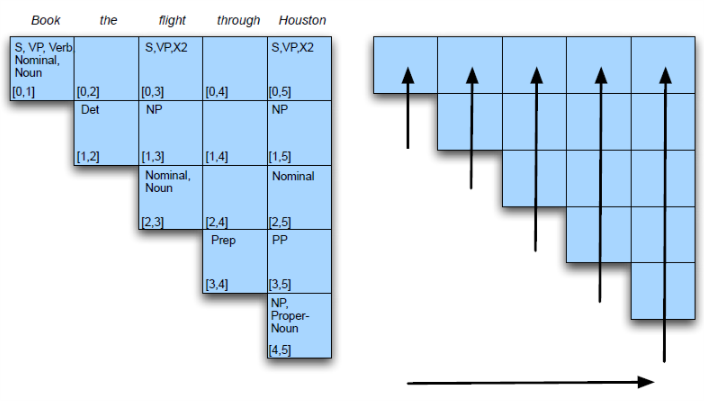
\includegraphics[width=\textwidth]{gfx/cky-beispiel.png} 
\caption{Links: Beispielmatrix für den \textit{CKY}-Algorithmus angewandt auf den Satz \textit{``Book the flight through Houston''}. Rechts: Füllrichtung der Matrix. Beides entnommen aus \cite[S. 473]{nlpGrundlagen}
}	
\label{fig:cky-beispiel}
\end{figure}

\begin{figure} [h]
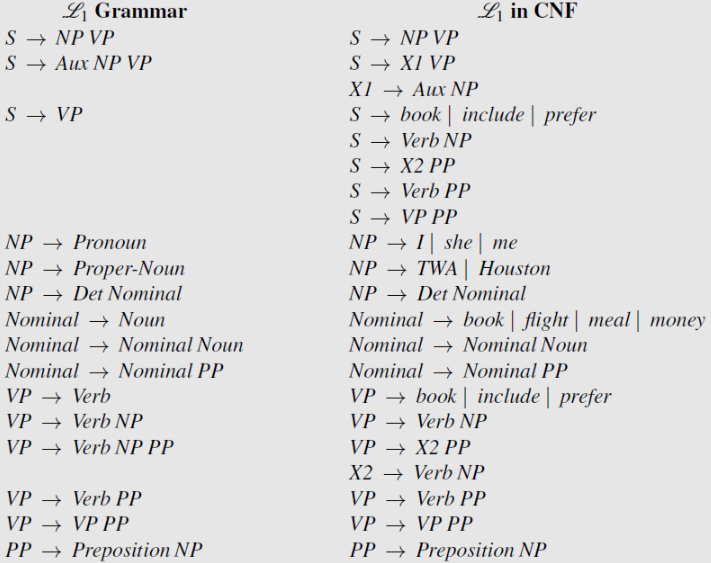
\includegraphics[width=\textwidth]{gfx/grammatik-cky-beispiel.png} 
\caption{Grammatik welche zum Parsen von \textit{``Book the flight through Houston''} verwendet wurde. Links in ursprünglicher Form, rechts in CNF. Entnommen aus \cite[S. 472]{nlpGrundlagen}
}	
\label{fig:cky-beispiel}
\end{figure}

Ohne zusätzliche Informationen gibt die Tabelle nur an, ob ein Satz grammatikalisch korrekt ist. Ein Satz ist korrekt, wenn in Zelle \([0, n]\) das Startsymbol steht. Um die verwendeten Regeln, also den Baum, bzw. die Bäume zur Eingabe zu erhalten, muss der Algorithmus erweitert werden. Die Erweiterung besteht darin, zu jedem Nichtterminal in jeder Zelle zusätzlich zu speichern, aus welchen zwei anderen Nichtterminalen es entstanden ist. Darüber hinaus darf das gleiche Nichtterminal mehrmals in einer Zelle vorkommen, da es aus unterschiedlichen Nichtterminalen entstanden sein kann. Ein Beispiel zur Tabelle in Abbildung \ref{fig:cky-beispiel} ist in Zelle \([0, 5]\) das Symbol \textit{S}. Es gibt drei Möglichkeiten dieses zu erzeugen: 
\begin{align}
& [0, 1]:Verb \; und\; [1, 5]:NP \nonumber \\ & [0, 3]:VP \; und \; [3, 5]:PP \nonumber \\ & [0, 3]:X2 \; und \; [3, 5]:PP \nonumber
\end{align}
Damit ergeben sich für die Eingabe drei verschiedene Syntaxbäume. Diese werden erstellt, indem man die Tabelle, beginnend mit dem jeweiligen Startsymbol, rückwärts durchläuft.

\section{Statistisches Parsen}
\label{sec:nlp:stat-parsen}

In diesem Abschnitt werden Mittel vorgestellt, welche dem Parser helfen sich zwischen mehreren, grammatikalisch korrekten Bäumen eines Eingabesatzes zu entscheiden. Hierfür benötigt der Parser für jeden errechneten Baum zusätzlich die Wahrscheinlichkeit, mit welcher dieser semantisch korrekt ist. Das heißt, jede Lösung ist mit einer Wahrscheinlichkeit versehen und es kann diejenige, deren Wert am höchsten ist als Lösung gewählt werden. %TODO letzten Satz evtl raus nehmen und ausführlich bei PCFG erklären

\subsection{Probabilistische Kontextfreie Grammatiken}
\label{sec:nlp:stat-parsen:pcfg}

Die Anforderung, einem Baum eine Wahrscheinlichkeit zuzuweisen, lässt sich mit dem Konzept der probabilistischen kontextfreien Grammatiken (kurz \textit{PCFG}) umsetzen. Abgesehen von zwei Erweiterungen haben die Produktionen einer \textit{PCFG} die gleiche Form wie die der ursprünglichen kontextfreien Grammatik. Erstens wird jeder Regel eine Wahrscheinlichkeit \textit{p}, mit \( 0 \leq p \leq 1 \), hinzugefügt.
\begin{equation}
A \to \beta  [p]
\end{equation}
Diese gibt an, mit welcher Wahrscheinlichkeit die rechte Seite unter der Vorbedingung der linken Seite auftritt.
\begin{equation}
p := P(A \to \beta | A)
\end{equation}
Es handelt sich um eine bedingte Wahrscheinlichkeit.\\ 
Zweitens muss für jedes Nichtterminal die Summe der Wahrscheinlichkeiten aller seiner Produktionen eins ergeben.
\begin{equation}
\sum_{\beta} P(A \to \beta) = 1
\end{equation}
Die Wahrscheinlichkeit für einen Baum errechnet sich dann durch das Produkt der Wahrscheinlichkeiten aller verwendeten Regeln. Eine Grammatik ist konsistent, wenn die Summe der Wahrscheinlichkeiten aller möglichen Sätze eins ergibt. Inkosistenz tritt auf, falls es eine Regel der Form \( A \to A \) gibt.\\
Mit dieser neuen Art von Grammatik ergeben sich auch neue Algorithmen zum Berechnen der Bäume. Sowohl der \textit{CKY}- als auch der \textit{Earley}-Algorithmus sind um den Faktor der Wahrscheinlichkeit erweiterbar, wobei der \textit{CKY}-Algorithmus mehr Verwendung findet. \\
Der in Kapitel \ref{sec:nlp:syn-parsen:cky} vorgestellte \textit{CKY}-Algorithmus wird dahingehend erweitert, dass in jeder Zelle für jedes Nichtterminal die Wahrscheinlichkeit gespeichert wird. Damit erhält man eine dreidimensionale \( (n+1) \times (n+1) \times V\) Matrix, wobei \textit{V} die Anzahl an Nichtterminalen in der Grammatik, und \textit{n} wie bisher die Anzahl an Wörtern im Satz, ist. \\
%TODO diesen Satz heraus nehmen oder so lassen oder CKY erklären, dann aber auch normalen kurz erklären...
Einen Nutzen kann man aus der zugefügten Wahrscheinlichkeit nur dann ziehen, wenn ihr numerischer Wert Sinn ergibt. Um diesen Wert für jede Regel zu berechnen, gibt es zwei Möglichkeiten. Zum einen kann dieser aus einer vollständig annotierten \textit{Treebank} errechnet werden. Hierfür wird jedes Auftreten einer Regel und des entsprechenden Nichtterminals gezählt und dividiert: 
\begin{equation}
P(A \to \beta) = \frac{Anzahl(A \to \beta)}{ \sum_{\gamma} Anzahl(A \to \gamma)} = \frac{Anzahl(A \to \beta)}{Anzahl(A)}
\end{equation}
Die Grammatik wird also anhand der annotierten Sätze der \textit{Treebank} trainiert. Die verwendeten Sätze werden Trainingsdaten genannt. \\
Falls man keine solche \textit{Treebank} zur Verfügung hat, gibt es eine zweite Möglichkeit die Werte der \textit{PCFG} festzulegen. Hierzu arbeitet der Parser einen unannotierter Textkorpus durch und fügt die entsprechenden \textit{Tags} ein. Zu Beginn haben alle Produktionen eines Nichtterminals die selbe Wahrscheinlichkeit. Der Korpus wird iterativ durchlaufen und nach jedem Durchgang werden die Wahrscheinlichkeiten der Regeln angepasst. Das Anpassen passiert wie in der ersten vorgestellten Möglichkeit, da zu diesem Zeitpunkt eine annotierte \textit{Treebank} vorhanden ist. Das Verfahren endet, wenn die Wahrscheinlichkeiten konvergieren. \\
Die resultierenden Werte in der Grammatik hängen davon ab, mit welchem Korpus sie berechnet wurden. Hierbei spielen Größe und Textart eine große Rolle. Um beim Parsen eines Textes möglichst gute Ergebnisse zu erhalten, sollte der Parser eine \textit{PCFG} verwenden, welche mit einem Text des selben Genres erstellt wurde. So kann man beispielsweise mit einer \textit{Treebank} aus technischen Handbüchern, unabhängig von ihrer Größe, beim Parsen eines informellen, gesprochenen Dialogs keine guten Ergebnisse erwarten, da sich die Sprache zu sehr unterscheidet.\\ %TODO Paper suchen über auswirken der unterschiedlichen Treebank arten für Parser!! 'Die' Treebank gibt es nicht - Diese These be - oder widerlegen!
Außerdem weist dieses neue Konzept auch zwei Nachteile auf.
Das erste Problem der \textit{PCFG} ergibt sich aus der Kontextfreiheit. Die Wahrscheinlichkeit einer Produktion ist immer gleich, egal an welcher Stelle im Satz sie auftritt. In einer natürlichen Sprache ist das aber im Allgemeinen nicht der Fall. Beispielweise kann die gewählte Produktion einer Nominalphrase abhängig davon sein, ob die Phrase Objekt oder Subjekt des Satzes ist. Da diese Information ohne Weiteres nicht in der Grammatik berücksichtigt werden kann, muss der Mittelwert aus beiden Fällen gebildet werden. Dies führt dazu, dass entweder im Falle des Objekts oder des Subjekts häufig die falsche Regel angewendet wird. \\
Die zweite Schwachstelle ergibt sich daraus, dass die einzelnen Wörter eine zu kleine Rolle spielen. Als Beispiel hierfür dient die bereits erklärte Anbindungs-Mehrdeutigkeit aus Kapitel \ref{sec:nlp:syn-parsen}. Wiederum wird eine Präpositionalphrase betrachtet, welche entweder an eine Verbal- oder eine Nominalphrase angebunden wird. An welche von beiden hängt allein von der \textit{Treebank} ab. Dort kommt entweder die Produktion \[ VP  \to  \alpha \;\;  NP \;\; PP \] oder die Kombination aus \[ VP  \to  \alpha \;\; NP \] und \[ NP  \to  NP \;\; PP \] öfter vor. \( \alpha \) steht für eines der hier möglichen Verb-Nichtterminale, welches aber in beide Fällen immer das selbe ist und deswegen keine Rolle spielt. Wesentlich bessere Resultate sind hier erzielbar, wenn man das Verb aus \textit{VP}, das Nomen aus \textit{NP} und die Präposition aus \textit{PP} in die Entscheidungsfindung mit einbezieht. Es kann aus der \textit{Treebank} die Information gewonnen werden, ob die gegebene Präposition sich öfter auf das Nomen oder das Verb bezieht. Angenommen es gibt eine Präposition, die ausschließlich mit Verben in Verbindung steht. In der \textit{Treebank} sind es nun aber die Nominalphrasen, an welche öfter Präpositionalphrasen gebunden werden. Dann wird die eben angenommene Präposition mit einer \textit{PCFG}, welche mit der \textit{Treebank} errechnet wurde, immer falsch zugeordnet. \\ 
Diese Schwäche der \textit{PCFG} macht sich ebenso bei der Koordinations-Mehrdeutigkeit bemerkbar. Beim Verbinden von Phrasen durch Konjunktionen kann wieder die konkrete Konjunktion und die Beziehung zu den entsprechenden Wörtern der zu verbindenden Phrasen betrachtet werden. Hierzu dient wieder das Beispiel aus Abschnitt \ref{sec:nlp:syn-parsen}: \textit{``old men and women''}. Es könnte eine \textit{Treebank} die Information liefern, dass die Wörter \textit{``men''} und \textit{``women''} per \textit{``and''} öfter direkt miteinander verbunden werden, als dass nur eines von beiden das Adjektiv \textit{``old''} zugeordnet bekommt. \\
Eine mögliche Verbesserung der \textit{PCFG} ergibt sich durch das Erweitern der Nichtterminale um die Information wessen Kind es ist. Es wird ein \textit{NP} als \textit{NP\^{}S} geschrieben, wenn \textit{S} der Elternknoten ist, oder als \textit{NP\^{}VP}, wenn es \textit{VP} ist. Hierdurch ergeben sich zwei neue Regeln in der Grammatik und damit auch zwei neue Wahrscheinlichkeiten. Mit diesem Konzept kann dem Nichtterminal, obwohl die Kontextfreiheit im grammatikalischen Sinne nicht verletzt wird, ein Kontext gegeben werden. Allerdings wird, wenn jedes Nichtterminal für jeden möglichen Elternknoten eine neue Produktion erhält, die Grammatik enorm aufgeblasen. Nebeneffekt dieser neuen Größe ist, dass bei gleich bleibender \textit{Treebank} für jede Regel weniger Trainingsdaten zur Verfügung stehen und damit die erhaltenen Wahrscheinlichkeitswerte ungenauer sind. Für einen gegebenen annotierten Trainings-Korpus muss ein Split-and-Merge Algorithmus ausgeführt werden, der errechnet wie weit eine Aufteilung der Nichtterminale sinnvoll ist.

\subsection{Probabilistische Lexikalisierte Kontextfreie Grammatiken}
\label{sec:nlp:stat-parsen:plcfg}

Ein weiterer Ansatz, um bessere Parserergebnisse zu erhalten, ist das Lexikalisieren der Grammatik. Hierfür muss der Begriff des Kopfes, im Englischen \textit{Head}, eingeführt werden. Die Idee ist, dass jede syntaktische Einheit einen Kopf in Form eines Wortes aus dieser Einheit besitzt. Es wird das Wort genommen, welches ``im Satz am grammatikalisch wichtigsten ist'' \cite[S. 443]{nlpGrundlagen}. %TODO Def. einbauen und Seite 443 zitieren.
% Da jedes Nichtterminal einer syntaktischen Einheit oder einem POS-Tag entspricht, kann jedem Nichtterminal und jeder Produktion der Grammatik ein Kopf zugewiesen werden.
Für das Finden des richtiges Wortes gibt es verschiedene Schritte. Begonnen wird, indem jedes POS-Nichtterminal sein Kind als \textit{Head} wählt. Dieses Wort wird dann im Baum nach oben weitergegeben. Für jede syntaktische Einheit gibt es Regeln, anhand derer einer der Köpfe der Kinder ausgewählt und als eigener eingesetzt wird. Ein Beispiel ist der lexikalisierte Baum für den Satz \textit{workers dumped sacks into a bin}, dargestellt in Abbildung \ref{fig:lex-tree-dumped-sacks}. %TODO Ref Buch Seite 445
\\
\begin{figure}
\qtreecentertrue\Tree [.S(dumped) [.NP(workers) [.NNS(workers) workers ] ] [.VP(dumped) [.VDB(dumped) dumped ] [.NP(sacks) [.NNS(sacks) sacks ] ] [.PP(into) [.IN(into) into ] [.NP(bin) [.DT(a) a ] [.NN(bin) bin ] ] ] ] ]
\caption{Lexikalisierter Baum für den Satz \textit{``Workers dumped sacks into a bin''}, entnommen aus \cite[S. 445]{nlpGrundlagen}} %TODO Sseite finden und zitieren
\label{fig:lex-tree-dumped-sacks}
\end{figure}
Zusätzlich zum Kopfwort kann auch noch dessen POS-Tag abgespeichert werden. Somit wird beispielsweise \textit{S(dumped)} zu \textit{S(dumped, VBD)} und \textit{NNS(workers)} zu \textit{NNS(workers, NNS)}. Die Wahrscheinlichkeit der Regel 
\begin{equation}\label{eqn:lexikal-dumped-sacks}
VP(dumped, VBD)  \to  VBD(dumped, VBD) \;\;  NP(sacks, NNS) \;\; PP(into, IN) 
\end{equation} %TODO alle Formeln so bennen
ergibt sich wieder aus dem Inhalt der \textit{Treebank}, nämlich durch die Formel
\begin{equation}
\frac{Anzahl(VP(dumped, VBD)  \to  VBD(dumped, VBD) \;  NP(sacks, NNS) \; PP(into, IN))}{Anzahl(VP(dumped, VBD))} 
\end{equation}
Dieser Wert ist null, wenn der Korpus keinen Satz mit \textit{dumped} \textit{sacks} \textit{into} enthält. Existiert kein Satz in welchem sich \textit{VP(dumped, VBD)} finden lässt, so ist dieser Wert nicht definiert. \\
Aufgrund dieses Problems bedarf es anderer Berechnungsvorschriften, wie zum Beispiel \textit{Collins Model 1}, vorgestellt in \cite{collinsModel}. 
Es wird jede Produktion folgendermaßen betrachtet: \textit{H} ist der Kopf, \( L_i \) sind die Nichtterminale links und \( R_i \) die rechts davon. Alle Nichtterminale bleiben weiterhin lexikalisiert. Das Kopfwort wird mit \textit{h} bezeichnet. Damit ergibt sich die Form
\[ A \to L_n...L_1 H R_1...R_m \]
Zusätzlich wird an der Stelle \( L_{n+1} \) und \( R_{m+1} \) das Nichtterminal \textit{STOP} eingefügt um anzuzeigen, dass hiernach die Regel zu Ende ist. In drei Schritten wird die Wahrscheinlichkeit der Produktion errechnet:
\begin{enumerate}
\item Es wird der Kopf mit der Wahrscheinlichkeit \( P_H(H | A, h) \) generiert.
\item Alle Elemente rechts vom Kopf werden mit \( \displaystyle\prod_{i = 1}^{m+1} P_R(R_i | A, h, H) \), also einschließlich dem \textit{STOP}, generiert.
\item Alle Elemente links von \textit{H} werden mit \( \displaystyle\prod_{i = 1}^{n+1} P_L(L_i | A, h, H) \) generiert.
\end{enumerate}
Für die Regel (\ref{eqn:lexikal-dumped-sacks}) errechnet sich die Wahrscheinlichkeit über
\begin{align}
P & = P_H(VBD|VP, dumped) \nonumber \\ & \times P_R(NP(sacks, NNS)|VP, dumped, VBD) \nonumber \\ & \times P_R(PP(into, IN)|VP, dumped, VBD) \nonumber \\ & \times P_R(STOP|VP, dumped, VBD) \nonumber \\ & \times P_L(STOP|VP, dumped, VBD)
\end{align}
Im Gegensatz zu vorher muss nicht die Kombination aus \textit{NP(sacks, NNS)}, \textit{PP(into, IN)} und \textit{VBD(dumped, VBD)} vorhanden sein. Es genügt, wenn jedes einzeln, als Kind von \textit{VP(dumped, VBD)} auf der entsprechenden Seite des \textit{Heads} in der \textit{Treebank} zu finden ist. %TODO eventuell erklären warum man das so machen kann: Markov, MLE, ... %TODO Distanz, Model 2 und 3 erklären?
Der Vollständigkeit halber ist außerdem zu erwähnen, dass dieses Modell um die Information der Distanz erweitert wird. Es wird zusätzlich berücksichtigt, wie weit ein Nichtterminal vom Kopf der Regel entfernt ist. 
Außerdem gibt es neben \textit{Model 1} noch zwei weitere Modelle. Diese Modelle bilden die Grundlage für den \textit{Collins Parser}. \cite{collinsModel}
% !TEX root = ../thesis-example.tex
%
\chapter{Konpzept}
\label{sec:konzept}

\section{Parser Input}

Die Eingabe des Parsers sind Sätze, die nach Tokens getrennt sind. Das heißt, alles was ein POS-Tag bekommt wird mit Leerzeichen getrennt. Ein solcher Satz wird \textit{sequenziert} genannt. Die meisten Wörter brauchen keine weitere Verarbeitung, da sie bereits ein Leerzeichen zum nächsten Wort haben. Ein typisches Beispiel für die Notwendigkeit der Aufteilung ist \textit{he's}, hier erkennt der Parser nur dass es sich um die Wörter \textit{he} und \textit{is} handelt, wenn ein Leerzeichen vor dem Apostroph eingeschoben wird. Bekommt man aus einem Korpus keine Version des Satzes, bei dem dieser Arbeitsschritt schon erledigt ist, muss man einen Tokenizer vorschalten. Hierfür gibt es unterschiedliche Anbieter, wie z.B. ...., %TODO Tokenizer suchen
allerdings wird in meiner Implementierung kein Tokenizer verwendet. Die Sätze der Eingabe müssen über ein Textdokument übergeben und zeilenweise getrennt sein. Der Parser erstellt für jede Zeile einen Baum.

\section{Parser Output}
Als Ausgabe gibt der Parser die annotierten Sätze in der Reihenfolge, in der sie eingegeben wurden, zurück. Es wird hierfür wieder ein Textdokument erstellt.% Bei manchen Parsern besteht die Möglichkeit für einen Satz die \textit{n} besten Bäume ausgeben zulassen. %TODO Entweder top n implementieren oder erklären wieso nicht implementiert und was man damit machen kann
Die annotierten Version des Satzes
\begin{quote}
It goes 150 miles an hour .
\end{quote}
lautet
\begin{quote}
( (S (NP (PRP It)) (VP (VBZ goes) (NP (NP (CD 150) (NNS miles)) \\(NP (DT an) (NN hour)))) (. .)) )
\end{quote}
Das äußerste Klammerpaar hat kein führendes Nichtterminal und könnte deshalb weggelassen werden. Es enthält typischerweise das Startsymbol der Parser, also \textit{ROOT}, \textit{TOP} oder ähnliches. Dieses wird aber für die Evaluierung aus dem Ergebnisbaum herausgenommen, weil es keine syntaktische Information liefert. Da der Satz des Goldstandards ebenfalls diese unannotierten Klammern besitzt, werden sie aus beiden Bäumen nicht gelöscht sondern später einfach ignoriert.
\section{Parser Modell}
Ein Parser erzielt, je nachdem welches Modell ihm zu Grunde liegt, sehr unterschiedliche Ergebnisse. Daher ist dieses Modell nicht fest im Parser verankert, sondern wird ihm als Datei übergeben. Somit kann man selbst Modelle anhand einer Treebank erstellen lassen um dann beispielsweise auf einem Parser die unterschiedlichen Modelle vergleichen. %TODO für die verwendeten Parser gibt es bereits erstelle Modelle die mit der ... Treebank trainiert wurden. Diese werden eingesetzt.

\section{Goldstandard}
Der Goldstandard sind die von Menschenhand erstellten Bäume zu den Sätzen der Eingabe. Es muss also für ein eingegebenes Textdokument, welches vom Parser bearbeitet werden soll auch ein Textdokument geben, das für jeden dieser Sätze die annotierte Version enthält. Die gratis verfügbaren Treebanks weisen oft ein unterschiedliches Sortiment an Dateien auf.\\
Der in dieser Arbeit verwendete Korpus heißt "The NAIST-NTT TED Talk Treebank". %TODO zitat paper treebank und ein zwei Sätze über diesen verlieren
Hier gibt es für jeden Satz eine Rohversion, eine sequenzierte und eine annotierte Version. Da es sich bei den Texten um Gespräche handelt sind sogar noch weitere Informationen, wie zum Beispiel Dauer und ähnliches vorhanden. Das wird hier aber nicht weiter verwendet. Falls man das Problem hat, dass nur die korrekten Lösungsbäume zur Eingabe verfügbar sind, so kann man sich z.B. mit NLTK %TODO Nltk verlinken
die Blätter jedes Lösungsbaums ausgeben lassen. Hierdurch erhält man, den in seine Token aufgeteilten Satz.\\
Ist der Lösungsbaum nicht einzeilig, sondern erstreckt sich ähnlich zu \ref{eqn:multiline-annotated-dog-eating}  über mehrere Zeilen, so muss hier auch eine Vorverarbeitung geschehen. Entweder kann anhand der Klammerung erkannt werden wo die Grenzen des Baumes liegen oder es müssen alle Zeilen, die mit einer Art Leerzeichen (Tabulator, u.ä.) beginnen, an die vorherige gehangen werden.

\section{Parser}

Alle Parser erhalten die Eingabe in selber Form, allerdings kann jeder Parser noch eine individuelle Vorverarbeitung benötigen. Dazu mehr in Abschnitt ... . %TODO ref Kapitel impl:parser
%TODO erklären dass keine Dependency parser verwendet werden und was das ist, erklären dass alle selbes Tagset verwenden und das keine relational tags verwendet werden

\subsection{Stanford Parser}

\subsection{Berkeley Parser}

\subsection{OpenNLP Parser}

\section{Evaluierung}


% !TEX root = ../thesis-example.tex
%
\chapter{Implementierung}
\label{sec:impl}
Dieses Kapitel beschreibt, wie das Konzept aus Kapitel \ref{sec:konzept} umgesetzt wurde. Es wird sowohl auf die neu implementierten Operatoren, als auch auf die verwendeten, bereits existenten RapidMiner-Operatoren eingegangen. 

\section{RapidMiner Studio}
\label{sec:impl:rms}

Die Plattform für das Parser-Framework wurde auf RapidMiner Studio \cite{rmstudio} festgelegt. Hierbei handelt es sich um eine Data Science Plattform, in der Operatoren im Steckkasten-Prinzip zu einem Prozess verbunden werden. Beim Ausführen eines Prozesses werden alle Operatoren, entsprechend der Reihenfolge in der sie verbunden sind, durchlaufen. Zwischen diesen Operatoren können Daten in unterschiedlicher Form übergeben werden. Die Operatoren selbst führen verschiedene Aufgaben aus. Das eigentliche RapidMiner Studio bietet hauptsächlich Operatoren für die Verarbeitung von Tabellen an. Allerdings sind über den RapidMiner Marketplace auch eine Vielzahl von Erweiterungen erhältlich. Im Rahmen dieser Arbeit wird die \textit{Text-Processing-Extension} (Version 8.1.0) \cite{textExt} %TODO ref text processing ext, ref https://rapidminer.com/products/studio/ 
verwendet. Diese stellt einfache NLP-Funktionalitäten zur Verfügung. RapidMiner bietet zusätzlich die Möglichkeit eigene Operatoren zu programmieren, was im Rahmen dieser Arbeit auch genutzt wurde. Das RapidMiner Studio, die Erweiterungen und die eigenen Operatoren wurden in Java geschrieben. \\

\section{Verwendete Operatoren}
\label{sec:impl:vwo}

Hier werden die bereits bestehenden Operatoren beschrieben, welche im Prozess verwendet wurden.

Zum Einlesen des Parser-Modells wurde der Operator \textbf{Read File} aus dem Ordner \textit{Utility\textbackslash Files} verwendet. Dieser hat als Parameter den Pfad für die zu öffnende Datei. Er bietet einen Output-Port, über den die geöffnete Datei später als \texttt{com.rapidminer.operator.nio.file.SimpleFileObject} verarbeitet werden kann. Das Dateiformat der Modelle ist \textit{.bin} für den OpenNLP-Parser, \textit{.gr} für den Berkeley-Parser und \textit{.ser.gz} für den Stanford-Parser. Wichtig ist hier aber nicht die geöffnete Datei, da alle Parser diese selbst nochmal öffnen. Die Parser bekommen als Übergabe den Pfad und dieser kann aus dem \texttt{SimpleFileObject} entnommen werden.

Aus der Text-Processing-Extension wird der Operator \textbf{Read Document} verwendet. Er wird an zwei Stellen verwendet. Zum einen wird über ihn der Input-Text für den Parser eingelesen. Zum anderen wird der \textit{Goldstandard} für die Evaluierung damit in den Prozess gebracht. In beiden Fällen wird nur der Parameter \textit{file} auf den entsprechenden Dateipfad gesetzt und alle anderen Parameter auf ihrem Default-Wert belassen. Auch sein Input-Port wird nicht verwendet. Über den Output-Port wird die geöffnete Datei als \texttt{com.rapidminer.operator.text.Document} an die nachfolgenden Operatoren übergeben.

Der letzte verwendete Operator ist \textbf{Execute Script} aus dem Ordner \textit{Utility\textbackslash Scripting}. Dessen Aufgabe ist das Ausführen von Java Code. Verwendung findet er lediglich in Kombination mit dem Stanford-Parser. Die verwendeten Pakete von Stanford werden hier einmal initialisiert, da es sonst einen Fehler seitens RapidMiner gibt. Hierfür wird ein Objekt der Klasse  \texttt{edu.stanford.nlp.trees.TreebankLanguagePack} erstellt und wieder auf \texttt{null} gesetzt. Weder die Input- noch die Output Ports des Operators werden genutzt, wodurch er vor den anderen Operatoren ausgeführt wird, und die Stanford-Pakete korrekt initialisiert werden. Um diese Strategie der Fehlerumgehung nutzen zu können, sind zwei zusätzliche Schritte notwendig. Zum einen muss die Datei \textit{stanford-parser.jar}, welche die entsprechenden Pakete beinhaltet, in den \textit{lib}-Ordner von RapidMiner Studio gelegt werden. Diesen findet man typischerweise unter \textit{Programme\textbackslash RapidMiner\textbackslash RapidMiner Studio\textbackslash  lib}. Das zweite und schwerwiegendere Problem ist der Bedarf einer Large License von RapidMiner. Mit der Lizenz in Kombination mit dem vorherigen Schritten wird der Fehler nicht geworfen. Anderweitig wird die Lizenz nicht benötigt. Für die Dauer dieser Arbeit wurde mir diese von RapidMiner kostenlos zur Verfügung gestellt.
\section{Eigene Operatoren}
\label{sec:impl:eigene}

Hier werden die Operatoren und alle dazugehörigen Klassen, die für dieses Parser-Framework entwickelt wurden, vorgestellt. 

Zur Entwicklung einer eigenen Erweiterung stellt RapidMiner eine Anleitung zur Verfügung \cite{rmguide}. %TODO ref https://docs.rapidminer.com/latest/developers/creating-your-own-extension/ 
Als Entwicklungsumgebung wurde Eclipse (Version: Oxygen.3a Release (4.7.3a)) in Kombination mit dem Gradle Plugin  gewählt. 

Alle entwickelten Operatoren erben von der Klasse \texttt{com.rapidminer.operator.Operator} und die Methode \texttt{doWork()} wird aufgerufen, wenn der Operator im Prozess durchlaufen wird. 

Die Übergabe von Daten zwischen Operatoren erfolgt über Klassen, die das Interface \texttt{com.rapidminer.operator.IOObject} implementieren, wie z.B. \texttt{ExampleSet} oder \texttt{Document}. 

Im Rahmen dieser Arbeit wurden folgende Operatoren erstellt: \textbf{Berkeley Parser}, \textbf{OpenNLP Parser}, \textbf{Stanford Parser}, \textbf{Compare Results} und \textbf{Show Results}

Alle Parser-Operatoren haben die gleichen Ports zur Ein- und Ausgabe. 
\begin{description}
\item[ioobjectInputGrammar]
Über diesen Port wird das Modell des Parsers eingelesen. Dieses wird in \texttt{doWork()} auf ein \texttt{SimpleFileObject} gecastet, um den Dateipfad auslesen zu können. Er wird mit dem Read-File-Operator verbunden.
\item[ioobjectInputText] Hier liest der Operator den Input-Text für den Parser ein. Das \texttt{IOObject} wird auf ein \texttt{Document} gecastet, um den Inhalt als String zu bekommen. Dieser String wird dann nach Zeilen getrennt, da jeder Parser immer eine Zeile eingegeben bekommt. Er wird mit dem Read-Document-Operator verbunden.
\item[nameOutputExt] Es wurde ein PortExtender verwendet. Das heißt, falls man diesen Port verbindet wird der selbe Port nochmals erstellt. Somit kann man die Parser Ausgabe öfters verwerten. Dies kann man z.B. nutzen, um in der Evaluation unterschiedliche Paramter zu setzen. Extender müssen im Konstruktor des Operators mit der Methode \texttt{start()} aktiviert werden. Über die von diesem Extender erstellten Ports wird der Name des Parsers in einem \texttt{Document} nach außen gegeben. Hierfür gibt es einen Konstruktor der Klasse Document dessen Übergabeparameter ein String ist. 
\item[resultOutputExt] Dieser Extender gibt den geparsten Text in einem \texttt{Document} aus. Hier sind alle einzeln verarbeiteten Zeilen wieder zu einem String zusammen gefügt worden.
\end{description}

Für zukünftiges Einbringen von weiteren Parsern ist zu beachten, dass diese die gleichen Ports anbieten müssen und an diese auch Objekte der gleichen Form liefern müssen.

\subsection{Berkeley-Parser}

Der Code für diesen Parser ist aus der Klasse \texttt{edu.berkeley.nlp.PCFGLA.BerkeleyParser} entnommen. Diese Klasse wird beim Kommandozeilenaufruf des Parsers angesprochen. Die \texttt{main}-Methode sowie \texttt{outputTrees(...)} wurden leicht abgewandelt übernommen. 

Die Funktionalität der \texttt{main} wurde in die \texttt{doWork()} geschrieben. Über den eigentlichen Kommandozeilenaufruf können Optionen übergeben werden, die in ein Objekt der Klasse \texttt{edu.berkeley.nlp.PCFGLA.BerkeleyParser.Options} geparst werden. Hier wird stattdessen ein Objekt dieser Klasse erstellt und die Optionen manuell gesetzt. Der Wert des Attributs \texttt{grFileName} wird auf den Dateipfad des eingelesenen Modells gesetzt. Bei allen anderen werden die Default-Werte beibehalten.\\ 
Die Ein- und Ausgabe in der Originalklasse war ein \texttt{BufferedReader} und ein \texttt{PrintWriter}. Das wurde abgewandelt, da die Eingabe jetzt zeilenweise als String zur Verfügung steht und die Ausgabe auch in einen String geschrieben werden soll. Der Parser bekommt seine Eingabe jetzt über eine \texttt{for}-Schleife, in der über das Array der Eingabesätze iteriert wird. Zuvor wurden per \texttt{while}-Schleife und die BufferedReader Methode \texttt{readLine()} der Parser-Input erhalten.

Die Methode \texttt{outputTrees(...)} wurde als Methode des Operators aufgenommen. Hierzu wurde der Rückgabetyp von \texttt{void} auf \texttt{String} geändert und der Übergabeparameter zur Datenausgabe von \texttt{PrintWriter} auf \texttt{String} abgeändert. Das führt dazu, dass statt \texttt{outputData.write("...")} nun \texttt{outputText += "..."} verwendet wird. Außerdem wird die Möglichkeit, die Ausgabe als .png zu erhalten, entfernt. Zuletzt wird der Methode ein \texttt{return outputText} angehängt. In der \texttt{doWork()} wird dieser String als \texttt{Document} verpackt und über den PortExtender an die Output-Ports geliefert.

\subsection{OpenNLP-Parser}
\label{sec:impl:eigene:opennlp}

OpenNLP bietet eine Anleitung zum Integrieren des Parsers in eine Anwendung mit Hilfe seiner API, zu finden unter \cite{openNlpManual}. %TODO ref http://opennlp.apache.org/docs/1.9.1/manual/opennlp.html#tools.parser
Der Code aus dieser Anleitung wurde in die \texttt{doWork()} des Operator geschrieben. Dieser Code wurde von einem zusätzlichen \texttt{try-catch}-Block umgeben, um eine \texttt{FileNotFoundException} zu fangen. Diese Exception wird beim Öffnen der Datei des Parser-Modells geworfen. Per \texttt{for}-Schleife werden die Sätze der Eingabe in den Parser geschickt. 

Über die String Methode \texttt{outputText.replaceAll("\textbackslash \textbackslash (TOP ", "( ");} wird das Startsymbol des Parsers entfernt. Um zu verhindern, dass das Auftreten des Wortes ``TOP'' im Eingabesatz gelöscht wird, wurde die Klammer mit in den regulären Ausdruck aufgenommen. Worte des Satzes haben in der Formatierung immer eine schließende Klammer nach sich, aber nie eine öffnende vorher. Deshalb wird so nur das Startsymbol entfernt.

\subsection{Stanford-Parser}

Beim Herunterladen des Parsers wird eine Demo-Klasse mitgeliefert, in welcher der Code zum Starten des Parsers aufgeführt wird. Hieraus wurden die notwendigen Befehle in die Methode \texttt{doWork()} des Operators übernommen. Zu beachten ist hier, dass der Parser den Satz nicht als \texttt{String} entgegen nimmt, sondern die Token des Satzes in einem \texttt{String}-Array.

Das Startsymbol dieses Parser lautet ``ROOT'' und wird analog zum OpenNLP-Parser aus \ref{sec:impl:eigene:opennlp} entfernt.

\subsection{Compare Results}

In diesem Operator findet die Evaluierung statt. Es wird die Ausgabe von genau einem Parser mit dem \textit{Goldstandard} verglichen und die Kennzahlen errechnet.

Hierzu gibt es drei Input-Ports, deren \texttt{IOObject} jeweils zu einem \texttt{Document} gecastet wird. Der erste Port erhält den Namen des Parsers, der zweite die Ausgabe der Parser und der dritte den \textit{Goldstandard}. Das Ergebnis wird in einem einzeiligen  \texttt{com.rapidminer.example.ExampleSet} ausgegeben. Dadurch kann man später mehrere Evaluierungen in einer Tabelle untereinander anzeigen lassen. 

Der Operator hat zwei \texttt{Boolean}-Parameter. \texttt{PARAMETER\_REMOVE\_SUFFIX} gibt an, ob den syntaktischen Tags die Suffixe entfernt werden sollen. Das heißt, dass NP-SBJ als NP gewertet wird. \texttt{PARAMETER\_COUNT\_ONLY\_SYNTACTIC\_TAGS} entscheidet ob alle Tags oder nur die syntaktischen in die Bewertung zählen. Die Parameter wurden entsprechend dem Extension Manual \cite{rmguide} erstellt. Default-Wert bezüglich der Suffixe ist \texttt{true} und bezüglich der syntaktischen Tags \texttt{false}.

Für die Evaluierung benötigt dieser Operator zwei zusätzliche Hilfsstrukturen. Zum einen das Enum \textbf{PennTag}. Hier sind alle Tags der Penn Treebank aufgelistet. Jedes Literal hat einen String als Attribut, der die Schreibweise angibt. Somit kann über die statische Methode \texttt{stringToPennTag(String s, boolean removeSuffix)} ein String auf ein Enum-Literal abgebildet werden. Hierzu werden alle Tags durchlaufen und deren Attribut mit dem Übergabestring verglichen. Das entsprechende Literal wird zurückgegeben. Für den Fall, dass dem String kein Tag entspricht, wird das zusätzlich eingeführte Literal \texttt{Empty}, mit leerem String als Attribut, zurückgegeben. Das passiert beispielsweise dann, wenn im Parser oder \textit{Goldstandard} zusätzliche Tags verwendet werden. Eine Konstituente, die als Typ \texttt{Empty} hat, wird immer als falsch gewertet. \texttt{removeSuffix} sorgt dafür, dass die Tags ab dem ersten Bindestrich abgeschnitten werden und somit nur das ursprüngliche betrachtet wird. \\
Zum anderen wird die Klasse \textbf{ParseTreeNode} verwendet. Ein Objekt dieser Klasse entspricht einer Konstituente aus Kapitel \ref{sec:konzept:eval}. Realisiert wurde dieses Konzept über ein \texttt{PennTag} und zwei \texttt{int} Membervariablen für den Typ und die Grenzen. Über die Methode \texttt{equals(Object obj)} wird getestet, ob sowohl Tag, als auch Grenzen des übergebenen \texttt{ParseTreeNodes} mit dem aufrufendem übereinstimmen. 

Der Operator selbst bedient sich wiederum zweier Hilfsmethoden. Mit 

\texttt{private static String formatSentence(String s)} 

wird jede Zeile so formatiert, dass vor und hinter jeder Klammer ein Leerzeichen ist. Außerdem gibt es keine aufeinanderfolgenden Leerzeichen. Dadurch kann der String nach Leerzeichen geteilt werden. Durch

\texttt{private static List<ParseTreeNode> parseSentence(String s, boolean removeSuffix, boolean countOnlySyntacticTags)}

wird eine formatierte Zeile \texttt{s} in eine Liste von Konstituenten umgewandelt. Hierfür wird ein \texttt{Stack<ParseTreeNode>} genutzt. Der Satz wird nach Leerzeichen in Klammern, Nichtterminale und Terminale aufgeteilt. Diese werden mit einer \texttt{for}-Schleife durchlaufen. Damit ergeben sich vier Fälle. 
\begin{itemize}
\item Fall 1: Öffnende Klammer. Es wird ein neuer \texttt{ParseTreeNode} erstellt und dessen Startpunkt auf die aktuelle Wortposition im Satz gesetzt. Diese Konstituente wird auf den Stack gelegt.
\item Fall 2: Nichtterminal. Die oberste Konstituente des Stacks wird geholt, ihr Typ auf das gelesene Nichtterminal gesetzt und sie selbst wieder auf den Stack zurückgelegt.
\item Fall 3: Terminal. Der Wortzähler wird inkrementiert. Das eigentliche Terminal wird nirgends abgespeichert, da diese in der Parser-Ausgabe und im \textit{Goldstandard} identisch sind. 
\item Fall 4: Schließende Klammer. Der oberste \texttt{ParseTreeNode} wird vom Stack geholt und sein Endpunkt auf den aktuellen Stand des Wortzählers gesetzt. Gilt \texttt{countOnlySyntacticTags == true}, so werden nur diejenigen \texttt{ParseTreeNodes} an die Ausgabe gehängt, deren \texttt{PennTag} zu den syntaktischen Tags gehört. Falls nicht, so wird jede Konstituente der Ausgabeliste hinzugefügt.
\end{itemize}
Diese Methode gibt alle zu bewertenden Konstituenten des Satzes zurück. 

In der \texttt{doWork()} des Operators werden sowohl Parser-Ausgabe, als auch \textit{Goldstandard} nach Zeilen aufgeteilt. Für jede Zeile der beiden Versionen werden die beschriebenen Hilfsmethoden aufgerufen. Die Parser-Konstituenten werden durchlaufen und im \textit{Goldstandard} nach passendem Gegenstück gesucht. Hierdurch bekommt man die Anzahl an korrekten Konstituenten. Für den \textit{RCB}-Wert werden nochmals die \texttt{ParseTreeNodes} des Parsers durchlaufen und alle gezählt, die mindestens eine Konstituente des \textit{Goldstandards} kreuzen. Diese beiden Zahlen, sowie die Anzahl an Parser- und \textit{Goldstandard}-Konstituenten werden für jede Zeile aufsummiert. Dadurch können, nach dem Vergleich aller Zeilen, entsprechend der Formeln (\ref{eqn:precision}) bis (\ref{eqn:rcb}), die Kennzahlen für den Parser errechnet werden. \\
Zuletzt wird ein \texttt{ExampleSet} mit den Attributen \texttt{Name, Precision, Recall, F1, Crossing Brackets}, sowie der totalen Anzahlen der Konstitueten, aus denen die Kennzahlen berechnet wurden, erstellt. Diese eine Zeile mit den Werten des Parser, wird in dieses Set eingefügt, welches dann an den OutputPort übergeben wird. 

\subsection{Show Results}

Dieser Operator dient lediglich dem Zusammenführen von mehreren Parser-Evaluationen. 

Es wird für die Input-Ports wieder ein PortExtender verwendet, um beliebig viele Compare-Results-Operatoren anschließen zu können. Der Output-Port liefert eine Tabelle, in der pro Zeile die Ergebnisse eines Parsers stehen.

In der \texttt{doWork()} werden alle Input-Ports durchlaufen und die Werte in die Ergebnistabelle übertragen. Diese wird zuletzt an den Output-Port geliefert.


\section{Prozess zum Evaluieren der Parser}

Mit den vorgestellten Operatoren lässt sich im RapidMiner Studio nun ein Prozess zum Evaluieren der Parser erstellen. Die Anordnung der Operatoren zur Evaluierung des Berkeley-Parsers wird in Abbildung \ref{fig:screenshot-prozess} präsentiert. Dieser Aufbau ist für alle Parser gleich. Lediglich bei \textbf{Read Grammar} muss beachtet werden, dass das entsprechende Modell geladen wird. Um mehrere Parser zu vergleichen,  muss das Konstrukt aus \textbf{Compare Results}, und allen links davon liegenden Operatoren, für die anderen Parser erstellt werden. Die Ausgänge der \textbf{Compare Results}-Operatoren werden mit \textbf{Show Results} verbunden. \\
Abbildung \ref{fig:results} zeigt einen Teil der Ausgabe des Prozesses beim Vergleich aller Parser. Nach dem Namen der Parser werden die vier Metriken aufgelistet. In der Abbildung wurden rechts vier Spalten entfernt, welche die Zahlen angeben, aus denen sich die Metriken berechnen. Diese Zahlen sollen unter anderem dabei helfen die Größe der geparsten Datei einzuordnen.

\begin{figure}
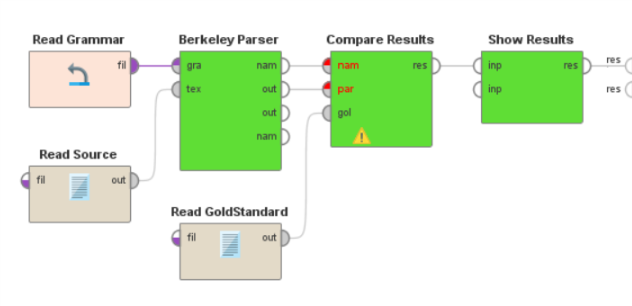
\includegraphics[width=\textwidth]{gfx/berkeley-skizze.png} 
\caption{RapidMiner-Prozess zur Evaluierung des Berkeley-Parsers}	
\label{fig:screenshot-prozess}	
\end{figure}

\begin{figure}
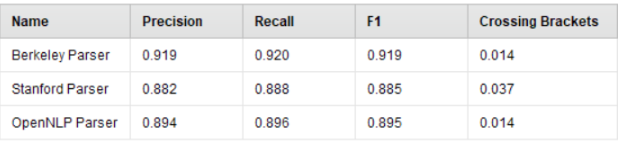
\includegraphics[width=\textwidth]{gfx/shortresults.png} 
\caption{Teil der Ausgabe des RapidMiner-Prozesses beim Vergleich aller Parser}	
\label{fig:results}	
\end{figure}

\section{Limitierung des Rahmenwerks}

Das Rahmenwerk besitzt auf Grund des zeitlichen Rahmens, der für diese Arbeit gesetzt war, noch Einschränkungen, die bei der Nutzung zu beachten sind. 

Der Eingabetext darf keine runden Klammern enthalten, da diese in der annotierten Version als Begrenzung einer Konstituente gesehen werden. Falls eine Klammer als Tag oder Terminal in der annotierten Version auftaucht, so wird sie nicht als dieses erkannt. 

Wie bereits in Abschnitt \ref{sec:impl:vwo} erwähnt, können der Stanford-Parser und RapidMiner nur unter gewissen Umständen zusammenarbeiten. Falls die nötigen Voraussetzungen nicht geschaffen werden können, muss der Stanford-Parser herausgelassen werden.

Um in den Parser-Operatoren das eingehende \texttt{IOObject} auf die Klasse \texttt{Document} zu casten, musste die Text-Processing-Erweiterung in der Rahmenwerk-Erweiterung eingebunden werden. Das führt dazu, dass beim Start von RapidMiner Studio eine Fehlermeldung bezüglich inkompatibler Erweiterungen erscheint. Diese erscheint, da RapidMiner versucht die Text-Processing-Erweiterung doppelt zu laden. Durch den Button \textit{Ignore} kann, ohne Auswirkungen, zum RapidMiner Studio fortgefahren werden.
 
% !TEX root = ../thesis-example.tex
%
\chapter{Evaluierung der Parser}
\label{sec:eval}

In diesem Kapitel wird die Funktionsweise der Parser vorgestellt. Danach wird die Leistung der Parser anhand der Ted-Talks-Treebank getestet und eine weitere Parser-Evaluation betrachtet.


\section{Stanford-Parser}
%TODO https://nlp.stanford.edu/nlp/javadoc/javanlp/edu/stanford/nlp/parser/lexparser/package-summary.html
Der Stanford-Parser bringt ein Modell namens \textit{englishPCFG} mit. Es handelt sich dabei um eine unlexikalisierte PCFG für die englische Sprache. 
\section{Berkeley-Parser}

\section{OpenNLP-Parser}


\section{Leistung der Parser}
Dieser Korpus enthält zehn Texte unterschiedlicher Länge, die alle von jedem Parser bearbeitet werden. In Tabelle \ref{tab:eval-parser} sind die Ergebnisse aufgeführt. Für die Messung wurden alle Tags gewertet, nicht nur die syntaktischen. In einer Zeile stehen die Werte für die entsprechende Datei. Für den totalen Wert wurde die Anzahl der unterschiedlichen Konstituenten über alle zehn Dateien aufsummiert und anhand dieser Zahlen nach entsprechender Formel berechnet. Somit wird die unterschiedliche Größe der Texte berücksichtigt. \\
Der Berkeley-Parser nimmt mit Precision- und Recall-Resultaten von über 93\% den ersten Platz ein. Der OpenNLP-Parser liegt, mit weniger als 1\% Vorsprung in beiden Werten, vor dem Stanford-Parser. Beide weisen einen gleich hohen Anteil an kreuzenden Konstituenten auf.\\
Für die Interpretation dieser Ergebnisse muss beachtet werden, dass die Modelle nicht mit den selben Texten trainiert wurden. Es handelt sich um die vortrainierten Modelle der Parser-Anbieter. Um aussagekräftigere Ergebnisse zu erhalten, müssen eigene Modelle erstellt werden. 
%TODO zeitmessung
\begin{sidewaystable}

\begin{tabular}{ | l || l | l | l | l || l | l | l | l || l | l | l | l |}
	\hline
	& \multicolumn{4}{|c||}{Berkeley Parser} & \multicolumn{4}{|c||}{Stanford Parser} & \multicolumn{4}{|c|}{OpenNLP Parser}\\ \hline
	Dateiname & Precision & Recall & \( F_1 \) & RCB & Precision & Recall & \( F_1 \) & RCB & Precision & Recall & \( F_1 \) & RCB  \\
	\hline \hline
	SheaHembrey\_2011 & 93,3\%  & 93,2\% & 93,2\% & 2,7\% & 89,4\% & 89,2\% & 89,3\% & 4,4\% & 89,9\% & 89,3\% & 89,6\% & 3,6\%\\ \hline
	RobertLang\_2008 & 93,8\% & 93,4\% & 93,6\% & 2,4\% & 89,4\% & 89,1\% & 89,3\% & 3,5\% & 89,2\% & 89,1\% & 89,2\% & 3,3\% \\ \hline
	JessaGamble\_2010G & 94,3\% & 94,4\% & 94,4\% & 2,2\% & 88,3\% & 89,6\% & 88,9\% & 3,8\% & 90,3\% & 90,3\% & 90,3\% & 2,9\% \\ \hline
	MihalyCsikszentmihaly\_2004 & 93,8\% & 93,0\% & 93,4\% & 3,8\% & 87,8\% & 85,2\% & 86,4\% & 6,0\% & 89,6\% & 89,1\% & 89,3\% & 5,5\% \\ \hline
	YvesBahar\_2009 & 91,9\% & 92,0\% & 91,9\% & 1,4\% & 88,2\% & 88,8\% & 88,5\% & 3,7\% & 89,4\% & 89,6\% & 89,5\% & 1,4\% \\ \hline
	KatherineFulton\_2007 & 92,8\% & 92,3\% & 92,5\% & 3,5\% & 85,7\% & 83,4\% & 84,5\% & 4,8\% & 87,2\% & 87,3\% & 87,2\% & 6,0\% \\ \hline
	HannaRosin\_2010W & 93,1\% & 92,8\% & 92,9\% & 4,1\% & 90,0\% & 89,3\% & 89,7\% & 4,2\% & 89,3\% & 88,5\% & 88,9\% & 4,8\% \\ \hline
	HansRosling\_2010S1 & 92,4\% & 92,6\% & 92,5\% & 2,9\% & 88,9\% & 89,6\% & 89,2\% & 3,6\% & 87,4\% & 87,2\% & 87,3\% & 4,4\% \\ \hline
	StefanaBroadbent\_2009G & 92,8\% & 92,1\% & 92,5\% & 3,8\% & 88,5\% & 88,0\% & 88,2\% & 5,6\% & 87,9\% & 87,8\% & 87,8\% & 5,5\% \\ \hline
	AnthonyAtala\_2009P & 94,5\% & 94,3\% & 94,4\% & 2,0\% & 89,0\% & 87,9\% & 88,4\% & 3,9\% & 90,3\% & 90,4\% & 90,3\% & 3,4\% \\ \hline \hline
	Total & 93,4\% & 93,1\% & 93,3\% & 3,0\% & 88,7\% & 87,9\% & 88,3\% & 4,4\% & 89,1\% & 88,8\% & 89,0\% & 4,4\% \\ \hline
\end{tabular}
\caption{Evaluation der Parser für die Ted-Talks-Treebank} 
\label{tab:eval-parser}
\end{sidewaystable} 

\section{Weitere Evaluationen}

%TODO
% !TEX root = ../thesis-example.tex
%
\chapter{Schluss}
\label{sec:schluss}

Zuletzt wird ein Fazit gezogen und ein Ausblick gegeben.

Die erstellte Erweiterung enthält alle notwendigen Operatoren um syntaktische NLP-Parser zu evaluieren und zu vergleichen. Die Parser-Operatoren können auch zum Zweck der Annotation eingesetzt werden, da ihre Ausgabe mit Hilfe der Text-Processing-Erweiterung als Datei abgespeichert werden kann. Für das Einbringen von weiteren Parsern ist, durch die bestehenden Operatoren eine Vorlage gegeben.

Des weiteren bietet dieses Rahmenwerk einige Punkte zur Weiterentwicklung.
\begin{description}
\item[Zeitmessung]
Für die Bewertung der Parser kann neben der Korrektheit auch noch die Geschwindigkeit einbezogen werden. 
\item[Modelle trainieren]
Oft bieten die Parser die Möglichkeit ein neues Modell anhand einer Treebank zu trainieren. Die Umsetzung dieses Features mittels RapidMiner-Operatoren würde das Evaluations-Rahmenwerk enorm bereichern. 
\item[Vorverarbeitung der Ergebnisse]
Für den Vergleich von Parser-Ausgabe und Goldstandard werden beispielsweise in \cite{parseval} Möglichkeiten zur Bearbeitung der annotierten Sätze vorgestellt. Diese können ins Rahmenwerk eingebracht, und dann mittels Parameter aktiviert oder deaktiviert werden.
\item[Dependenz-Parser]
Das Rahmenwerk beinhaltet aktuell nur Parser, welche die Konstituenten der Sätze errechnen. Sogenannte Dependenz-Parser geben die Abhängigkeiten der Wörter untereinander an. Eine mögliche Erweiterung ist das Einbringen des Vergleichs von Dependenz-Parsern.
\end{description}
\cleardoublepage

% --------------------------
% Back matter
% --------------------------
{%
\setstretch{1.1}
\renewcommand{\bibfont}{\normalfont\small}
\setlength{\biblabelsep}{0pt}
\setlength{\bibitemsep}{0.5\baselineskip plus 0.5\baselineskip}
\printbibliography[nottype=online]
\printbibliography[heading=subbibliography,title={Websites},type=online,prefixnumbers={@}]
}
\cleardoublepage

\listoffigures
\cleardoublepage

\listoftables
\cleardoublepage



% !TEX root = ../thesis-example.tex
%
%************************************************
% Declaration
%************************************************
\pdfbookmark[0]{Declaration}{Declaration}
\chapter*{Eidesstattliche Erklärung}
\label{sec:declaration}
\thispagestyle{empty}

Ich erkläre hiermit an Eides statt, dass ich die vorliegende Arbeit selbständig verfasst
und dabei keine anderen als die angegebenen Hilfsmittel benutzt habe. Sämtliche
Stellen der Arbeit, die im Wortlaut oder dem Sinn nach Publikationen oder Vorträgen
anderer Autoren entnommen sind, habe ich als solche kenntlich gemacht. Die Arbeit
wurde bisher weder gesamt noch in Teilen einer anderen Prüfungsbehörde vorgelegt
und auch noch nicht veröffentlicht.

\bigskip

\noindent\textit{\thesisUniversityCity, \thesisDate}

\smallskip

\begin{flushright}
	\begin{minipage}{5cm}
		\rule{\textwidth}{1pt}
		\centering\thesisName
	\end{minipage}
\end{flushright}

%*****************************************
%*****************************************

\clearpage
\newpage
\mbox{}

% **************************************************
% End of Document CONTENT
% **************************************************
\end{document}
